\documentclass[conference]{IEEEtran}
\usepackage{cite}
\usepackage{amsmath,amssymb}
\usepackage{graphicx}
\usepackage{booktabs}
\usepackage{array}
\usepackage[T1]{fontenc}
\usepackage{url}
\graphicspath{{../../results/figures/}}
\renewcommand{\arraystretch}{1.05}
\begin{document}
\title{Machine Learning-Based Smart Campus Energy Consumption Prediction and Anomaly Detection}
\author{\IEEEauthorblockN{Jahnavi Kallolini, Navya Menon, Keshav Agrawal}
\IEEEauthorblockA{B.Tech CSE (AI\&ML), School of Computer Engineering, Manipal Institute of Technology\\
Mentors: Dr. Narendra V. G., Dr. Ashwath Rao}}
\maketitle

\begin{abstract}
We study hourly electricity prediction and anomaly detection for seven campus buildings of the I-BLEND dataset. One model per building
is trained with Linear Regression, K-Nearest Neighbors, Decision Tree and Support Vector Regression (SVR) on calendar features, lagged power,
rolling statistics and lagged occupancy, using a chronological split (train 2014-02-17 to 2016-06-30, validation 2016-07-01 to 2016-12-31).
Hyper-parameters and encodings were chosen on validation only. SVR obtained the lowest macro-averaged standardized RMSE on validation (0.321,
macro R$^2$ 0.892) and on the primary test period 2017-01-01 to 2017-07-07 (0.382, R$^2$ 0.850), against 0.490 for a persistence baseline;
Linear Regression was close (0.392). Lagged occupancy did not improve accuracy beyond lagged power. Energy timestamps from July 2017 onward appear
displaced by roughly 4.5--5.5 hours relative to occupancy and to earlier years; the cause is unresolved, so the later part of the original test period is
reported only as a sensitivity analysis. Residual-based anomaly detection (modified z-score on validation residuals) flags 3.69\% of primary-test hours;
the flagged hours are statistical outliers and not confirmed faults. PCA and K-Means give an exploratory description of the feature space and of daily load profiles.
A Streamlit dashboard presents the saved results.
\end{abstract}
\begin{IEEEkeywords}
Smart Campus, Energy Consumption, Machine Learning, Energy Prediction, Anomaly Detection, Regression, PCA, K-Means
\end{IEEEkeywords}

\section{Introduction}
University campuses contain buildings with very different schedules and occupancy, so their electricity demand varies strongly with the hour, the weekday
and the academic calendar. Predicting the expected demand supports planning and benchmarking, and comparing measurements with the expected value highlights periods
that deserve inspection. This work follows a project synopsis that specifies the I-BLEND dataset~\cite{rashid2019iblend}, four regression algorithms, prediction-based
anomaly detection, PCA and K-Means. We aim at a transparent, leakage-free pipeline whose limitations are stated explicitly.

\section{Related Work}
Prior studies on campus and educational buildings have applied long short-term memory networks~\cite{faiq2023lstm}, conventional machine-learning regressors~\cite{elhabyb2024ml} and
support vector machines~\cite{liu2020svm} to consumption prediction. Occupancy-based consumption modelling for institutional buildings is studied in~\cite{anand2021occupancy},
PCA-based feature reduction for prediction models in~\cite{parhizkar2021pca}, and K-means clustering of consumers with smart-meter features in~\cite{okereke2023kmeans}.
Anomaly detection of building energy consumption has been reviewed in~\cite{himeur2021anomaly}. We do not compare our numbers with these works, because the datasets, targets and protocols differ.

\section{Dataset and Problem Formulation}
\subsection{I-BLEND}
I-BLEND contains electrical measurements of campus buildings of an Indian institute from August 2013 to December 2017~\cite{rashid2019iblend}. We use the seven main
feeders (Academic, Boys Hostel, Facilities, Girls Hostel, Lecture, Library, Mess) at one-minute resolution (power in watts, plus current, voltage, frequency and power factor),
the ten-minute occupancy counts derived from Wi-Fi data (each value is the maximum of the one-minute counts in its window), the daily academic calendar
(\texttt{working\_day} and \texttt{activity}, where H denotes high-activity and L low-activity periods) and a weather file. Each hostel also has a UPS (``backup'') feeder;
these two feeders are documented but excluded to keep the seven-building scope of the synopsis. The weather file covers only March--June 2018, after the last energy reading, so it cannot be aligned with the energy data and is not used.
Occupancy exists from 2014-02-16 to 2017-11-03. Missing minutes are absent rows; the seven mains are simultaneously present in only 42\% of minutes, so each building is modelled on its own valid data.

\subsection{Target and prediction setting}
The target is $y_t$, the mean of the valid one-minute power readings in the hour starting at $t$ (IST), valid if at least 45 of 60 readings exist. All predictors for hour $t$
use information available before $t$ (Section~IV-B), so the task is one-step-ahead prediction of the expected consumption of the coming hour.

\section{Methodology}
\subsection{Preprocessing}
Epoch timestamps were converted to IST (+05:30, no daylight saving). Hourly occupancy is the mean of the 10-minute counts present in the hour (at least 4 of 6). Nothing is interpolated in the targets.
Absent occupancy observations are kept missing and are never read as zero occupancy, because the released occupancy contains no zero values; rows whose occupancy lags are unavailable are excluded
from the primary matrix. For lag inputs only, a causal last-observation-carried-forward over at most one hour is allowed; a masking experiment showed that this beats the value of the previous day only for one-hour gaps in all seven buildings.
Table~\ref{tab:cov} gives the retained data. The number of valid hours changed little when the energy threshold was varied between 30 and 55 valid minutes (see \texttt{reports/preprocessing\_report.md}).

\begin{table}[t]
\caption{Valid hourly energy observations and rows of the primary matrix.}\label{tab:cov}
\centering\small
\begin{tabular}{lrrr}
\toprule
Building & Valid hours & \% of logging span & Primary rows\\
\midrule
Academic & 37{,}805 & 98.1 & 28{,}894 \\
Boys Hostel & 27{,}668 & 71.8 & 18{,}385 \\
Facilities & 34{,}039 & 94.1 & 23{,}739 \\
Girls Hostel & 27{,}482 & 71.3 & 18{,}392 \\
Lecture & 37{,}806 & 98.1 & 22{,}738 \\
Library & 28{,}547 & 74.1 & 18{,}831 \\
Mess & 33{,}513 & 89.5 & 25{,}353 \\
\bottomrule
\end{tabular}
\end{table}

\subsection{Features and leakage control}
Calendar features: hour, day of week, weekend flag, month, \texttt{working\_day}, \texttt{activity\_high} (the academic calendar is fixed in advance). History features:
$y_{t-1}$, $y_{t-2}$, $y_{t-24}$, and the mean and standard deviation of $y_{t-24},\dots,y_{t-1}$. Occupancy features: lagged occupancy at $t-1$, $t-2$, $t-24$ (never the occupancy of hour $t$).
Automated tests verify that lags equal the value at $t-k$ hours, that rolling windows use exactly $t-24$ to $t-1$, that changing the target at $t$ first affects the features at $t+1$, that scalers and one-hot categories are fitted on training rows only,
and that the tuning code never loads test rows.

\subsection{Split}
Train: 2014-02-17 to 2016-06-30 (90{,}640 rows); validation: 2016-07-01 to 2016-12-31 (28{,}428 rows); primary test: 2017-01-01 to 2017-07-07 (20{,}231 rows). The original test period extended to 2017-11-04
(37{,}264 rows); the part from 2017-07-11 (16{,}885 rows) is affected by the timestamp discontinuity (Section~VI-D) and is reported as sensitivity analysis.

\subsection{Regression models and selection}
One model per building and algorithm: Linear Regression (OLS), KNN regression, Decision Tree regression and SVR with an RBF kernel~\cite{drucker1997svr}, implemented with scikit-learn~\cite{pedregosa2011sklearn}.
KNN and SVR use standardized inputs (SVR also a standardized target). Temporal variables were tested with raw integer, sinusoidal (24, 7 and 12 periods) and one-hot encodings
(trees use raw integers). Encoding and hyper-parameters were selected on validation: for every candidate, models were fitted per building on training rows and scored on validation rows;
one configuration per algorithm and feature set was kept, the one with the lowest macro-average validation standardized RMSE (Table~\ref{tab:cfg}). SVR candidates were tuned on a chronological subsample of at most 3000 training rows per building and then refitted on all training rows.
The best algorithm was chosen on validation; test data were used once, after freezing, with models fitted on training rows only. Predictions are clipped at 0~W.
Metrics, with $n$ evaluation hours:
\begin{align}
\mathrm{MAE} &= \tfrac1n\textstyle\sum_i |y_i-\hat y_i|, \quad \mathrm{MSE} = \tfrac1n\sum_i (y_i-\hat y_i)^2,\\
\mathrm{RMSE} &= \sqrt{\mathrm{MSE}}, \quad R^2 = 1-\tfrac{\sum_i (y_i-\hat y_i)^2}{\sum_i (y_i-\bar y)^2},\\
\mathrm{nRMSE}_\sigma &= \mathrm{RMSE}/\sigma_{\mathrm{train}}, \quad \mathrm{nMAE}_\sigma = \mathrm{MAE}/\sigma_{\mathrm{train}} .
\end{align}
Because building scales differ by more than an order of magnitude, the macro average (equal weight per building) of $\mathrm{nRMSE}_\sigma$, $\mathrm{nMAE}_\sigma$ and $R^2$ is used for overall comparison; $\sigma_{\mathrm{train}}$ is the standard deviation of the building's training target.
Persistence ($\hat y_t=y_{t-1}$) and seasonal naive ($\hat y_t=y_{t-24}$) are reported as reference baselines, not as candidate models.

\begin{table}[t]
\caption{Configurations selected on validation (per feature set).}\label{tab:cfg}
\centering\small
\begin{tabular}{llll}
\toprule
Model & Features & Encoding & Hyper-parameters\\
\midrule
LR & energy+occ. & onehot & none \\
LR & energy-only & onehot & none \\
KNN & energy+occ. & onehot & k=20, weights=distance \\
KNN & energy-only & onehot & k=20, weights=distance \\
DT & energy+occ. & raw & max\_depth=8, min\_samples\_leaf=20 \\
DT & energy-only & raw & max\_depth=8, min\_samples\_leaf=20 \\
SVR & energy+occ. & onehot & C=30, gamma=0.005, epsilon=0.1 \\
SVR & energy-only & onehot & C=30, gamma=0.005, epsilon=0.1 \\

\bottomrule
\end{tabular}
\end{table}

\subsection{Anomaly detection}
Expected consumption is the model prediction $\hat y_t$ and the residual is $r_t=y_t-\hat y_t$. The modified z-score is
$z_t = 0.6745\,(r_t-\tilde r)/\mathrm{MAD}$, and hour $t$ is flagged as a \emph{potential anomalous consumption period} if $|z_t|>3.5$~\cite{iglewicz1993outliers}; $z_t>0$ means consumption above the expectation, $z_t<0$ below.
The median $\tilde r$ and the MAD are computed from \emph{validation} residuals only (out-of-sample for the models; training residuals are in-sample and understate future error), separately for each model, feature set, building,
day-part (night, morning, afternoon, evening) and operating regime (expected power below $0.25\,\sigma_{\mathrm{train}}$ or not). The MAD is not allowed to fall below $0.05\,\sigma_{\mathrm{train}}$; without this floor, Lecture's near-zero
residuals produced hundreds of spurious flags in a first run. The test period influences no threshold. No ground truth for faults exists in the data, so flagged hours are not evidence of equipment faults.

\subsection{PCA and K-Means}
PCA was fitted on training rows of the primary matrix (13 numeric features, standardized per building), for exploration only. K-Means~\cite{lloyd1982kmeans} was applied to building-days (24 valid hours, 2014-02-17 to 2016-12-31)
described by five shape features of the daily profile normalized by the building mean (mean, load factor, standard deviation, log day/night ratio, evening share); $K\in\{2,\dots,8\}$ was selected by the silhouette coefficient~\cite{rousseeuw1987silhouettes}.

\section{Experimental Setup}
Python 3.12.3, scikit-learn 1.8, pandas 3.0, NumPy 2.4, matplotlib 3.10; one CPU core of an Intel Xeon at 2.1~GHz, 4~GB RAM. The random seed is 42. Training seven SVR models takes about 56~s and seven Linear Regression models 0.2~s.
All code, tests and result tables are in the project repository; the pipeline and the model stage were re-run from scratch and reproduced the outputs.

\section{Results and Discussion}
\subsection{Model comparison}
Table~\ref{tab:val} and Table~\ref{tab:test} show macro averages over the seven buildings. On validation, SVR has the lowest error (nRMSE$_\sigma$ 0.321), followed by Linear Regression (0.348), Decision Tree (0.357) and KNN (0.398);
persistence reaches 0.442. On the primary test period the order of the best two is the same (SVR 0.382, Linear Regression 0.392), whereas Decision Tree (0.465) and KNN (0.464) are close to persistence (0.490).
The advantage of SVR over Linear Regression is small (about 0.01 in nRMSE$_\sigma$ on the primary test) and SVR is much more expensive to train and less interpretable.
Per-building results are in Tables~\ref{tab:pb} and~\ref{tab:r2}: Academic, Library and Facilities are the most predictable, the hostels and the Mess the least. Pooled errors in watts are dominated by the large buildings and should be read together with the standardized values.

\begin{table}[t]
\caption{Validation (2016-07-01 to 2016-12-31), macro average over seven buildings, primary features.}\label{tab:val}
\centering\small
\begin{tabular}{lrrr}
\toprule
Model & $R^2$ & nMAE$_\sigma$ & nRMSE$_\sigma$\\
\midrule
SVR & 0.892 & 0.207 & 0.321 \\
Linear Reg. & 0.877 & 0.230 & 0.348 \\
Decision Tree & 0.866 & 0.228 & 0.357 \\
KNN & 0.835 & 0.268 & 0.398 \\
Persistence (t-1) (baseline) & 0.805 & 0.262 & 0.442 \\
Seasonal naive (t-24) (baseline) & 0.487 & 0.420 & 0.710 \\

\bottomrule
\end{tabular}
\end{table}

\begin{table}[t]
\caption{Primary test (2017-01-01 to 2017-07-07), frozen models, macro average, primary features.}\label{tab:test}
\centering\small
\begin{tabular}{lrrr}
\toprule
Model & $R^2$ & nMAE$_\sigma$ & nRMSE$_\sigma$\\
\midrule
SVR & 0.850 & 0.230 & 0.382 \\
Linear Reg. & 0.845 & 0.247 & 0.392 \\
Decision Tree & 0.775 & 0.256 & 0.465 \\
KNN & 0.781 & 0.288 & 0.464 \\
Persistence (t-1) (baseline) & 0.760 & 0.288 & 0.490 \\
Seasonal naive (t-24) (baseline) & 0.389 & 0.442 & 0.781 \\

\bottomrule
\end{tabular}
\end{table}

\begin{table*}[t]
\caption{Per-building results of the selected model (SVR) and of Linear Regression (primary features). MAE and RMSE in W, MSE in $10^6$ W$^2$.}\label{tab:pb}
\centering\scriptsize
\begin{tabular}{llrrrrrrrr}
\toprule
 & & \multicolumn{4}{c}{Validation} & \multicolumn{4}{c}{Primary test}\\
\cmidrule(lr){3-6}\cmidrule(lr){7-10}
Building & Model & MAE & MSE & RMSE & $R^2$ & MAE & MSE & RMSE & $R^2$\\
\midrule
Academic & SVR & 1{,}797 & 8.70 & 2{,}949 & 0.960 & 1{,}733 & 8.28 & 2{,}878 & 0.956 \\
 & Linear Reg. & 2{,}362 & 14.05 & 3{,}748 & 0.936 & 2{,}326 & 13.54 & 3{,}679 & 0.928 \\
Boys Hostel & SVR & 1{,}844 & 8.66 & 2{,}943 & 0.852 & 2{,}629 & 14.47 & 3{,}804 & 0.814 \\
 & Linear Reg. & 1{,}930 & 9.17 & 3{,}029 & 0.844 & 2{,}524 & 13.94 & 3{,}733 & 0.821 \\
Facilities & SVR & 632 & 0.72 & 851 & 0.910 & 753 & 1.03 & 1{,}013 & 0.910 \\
 & Linear Reg. & 667 & 0.83 & 908 & 0.897 & 820 & 1.26 & 1{,}123 & 0.890 \\
Girls Hostel & SVR & 674 & 0.87 & 935 & 0.831 & 735 & 1.03 & 1{,}015 & 0.776 \\
 & Linear Reg. & 653 & 0.79 & 886 & 0.848 & 692 & 0.92 & 961 & 0.799 \\
Lecture & SVR & 200 & 0.23 & 475 & 0.915 & 306 & 1.01 & 1{,}005 & 0.744 \\
 & Linear Reg. & 282 & 0.32 & 568 & 0.878 & 348 & 0.82 & 904 & 0.793 \\
Library & SVR & 1{,}085 & 2.97 & 1{,}724 & 0.933 & 870 & 1.75 & 1{,}321 & 0.938 \\
 & Linear Reg. & 1{,}323 & 4.19 & 2{,}047 & 0.906 & 1{,}168 & 3.06 & 1{,}749 & 0.892 \\
Mess & SVR & 2{,}822 & 14.71 & 3{,}835 & 0.842 & 2{,}619 & 11.99 & 3{,}462 & 0.811 \\
 & Linear Reg. & 2{,}934 & 15.47 & 3{,}933 & 0.834 & 2{,}764 & 13.25 & 3{,}640 & 0.791 \\

\bottomrule
\end{tabular}
\end{table*}

\begin{table*}[t]
\caption{$R^2$ per building and model (primary features). SVR, LR = Linear Regression, DT = Decision Tree.}\label{tab:r2}
\centering\scriptsize
\begin{tabular}{lrrrrrrrr}
\toprule
 & \multicolumn{4}{c}{Validation} & \multicolumn{4}{c}{Primary test}\\
\cmidrule(lr){2-5}\cmidrule(lr){6-9}
Building & SVR & LR & DT & KNN & SVR & LR & DT & KNN\\
\midrule
Academic & 0.960 & 0.936 & 0.942 & 0.906 & 0.956 & 0.928 & 0.933 & 0.929 \\
Boys Hostel & 0.852 & 0.844 & 0.818 & 0.792 & 0.814 & 0.821 & 0.765 & 0.732 \\
Facilities & 0.910 & 0.897 & 0.877 & 0.817 & 0.910 & 0.890 & 0.728 & 0.835 \\
Girls Hostel & 0.831 & 0.848 & 0.811 & 0.790 & 0.776 & 0.799 & 0.753 & 0.715 \\
Lecture & 0.915 & 0.878 & 0.922 & 0.905 & 0.744 & 0.793 & 0.590 & 0.636 \\
Library & 0.933 & 0.906 & 0.900 & 0.877 & 0.938 & 0.892 & 0.898 & 0.881 \\
Mess & 0.842 & 0.834 & 0.796 & 0.758 & 0.811 & 0.791 & 0.756 & 0.741 \\

\bottomrule
\end{tabular}
\end{table*}

\begin{figure}[t]
\centering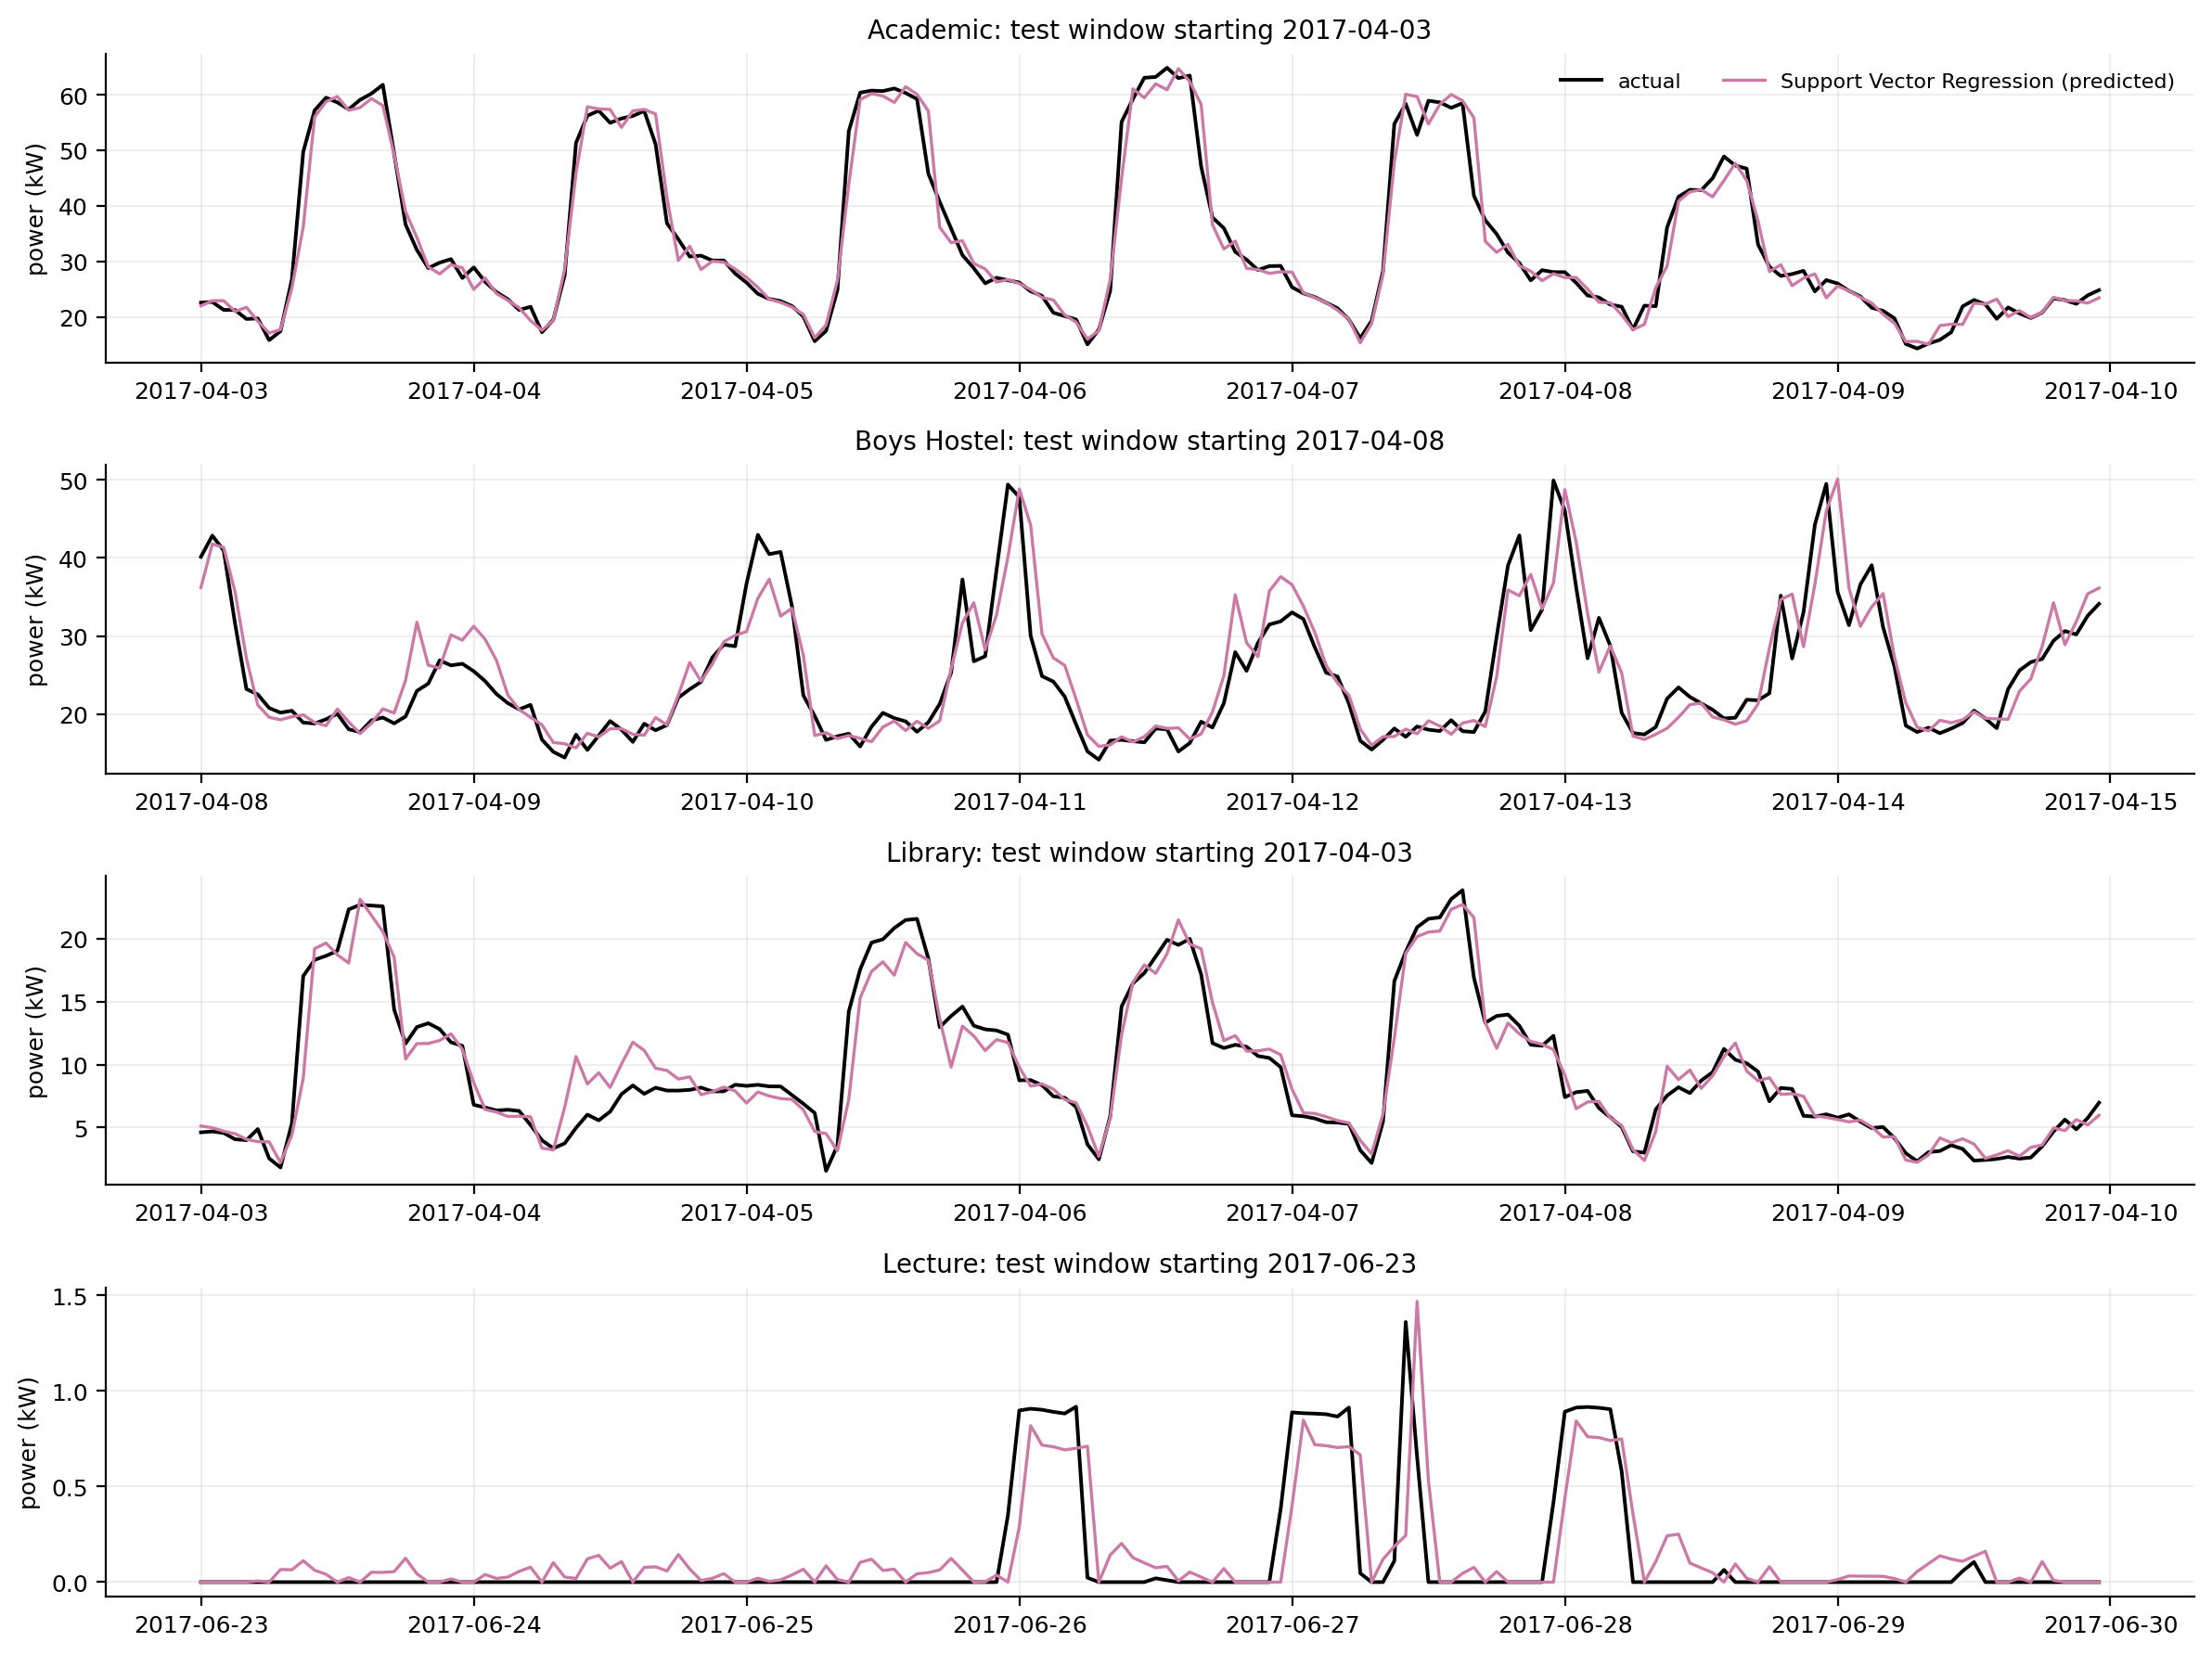
\includegraphics[width=\columnwidth]{fig12_actual_vs_predicted.png}
\caption{Actual and SVR-predicted hourly power in one-week windows of the test period (full test period figure; windows start after 3 April 2017).}\label{fig:avp}
\end{figure}

\subsection{Energy-only versus energy plus lagged occupancy}
Table~\ref{tab:fs} compares the feature sets. P uses energy and lagged occupancy; E-m uses energy features only, trained and scored on exactly the same rows; E-a is trained on all energy-only rows within the same dates and scored on the rows shared with P.
Lagged occupancy gives no measurable gain: for SVR and Linear Regression the energy-only and primary variants differ by at most 0.004 in nRMSE$_\sigma$, and energy-only is better for KNN and Decision Tree in both periods (for example KNN 0.372 versus 0.398 on validation). Lagged power already carries the occupancy-driven load pattern.
This does not show that occupancy is unrelated to load (same-hour Spearman correlations are 0.32--0.70 in the exploratory analysis), only that lagged occupancy adds no predictive skill beyond power lags in this setting. Training on all energy-only rows (E-a) helps KNN and Decision Tree slightly.

\begin{table*}[t]
\caption{Macro nRMSE$_\sigma$ by feature set on matched rows. P: energy + lagged occupancy; E-m: energy-only, same training rows; E-a: energy-only, all eligible training rows.}\label{tab:fs}
\centering\small
\begin{tabular}{lrrrrrr}
\toprule
 & \multicolumn{3}{c}{Validation} & \multicolumn{3}{c}{Primary test}\\
\cmidrule(lr){2-4}\cmidrule(lr){5-7}
Model & P & E-m & E-a & P & E-m & E-a\\
\midrule
SVR & 0.321 & 0.317 & 0.316 & 0.382 & 0.379 & 0.383 \\
Linear Reg. & 0.348 & 0.350 & 0.350 & 0.392 & 0.394 & 0.393 \\
Decision Tree & 0.357 & 0.355 & 0.355 & 0.465 & 0.454 & 0.453 \\
KNN & 0.398 & 0.372 & 0.369 & 0.464 & 0.447 & 0.446 \\

\bottomrule
\end{tabular}
\end{table*}

\subsection{Lecture building}
The Lecture feeder reads exactly 0~W in 82.5\% of the minutes and 79.3\% of the hours of the development window. Zero readings are strongly seasonal and calendar-dependent (above 99\% in March and December), occur in long runs (median run 3 min, but runs longer than a day contain 65\% of all zero minutes), and coincide with low occupancy; current is also 0 in most of them while the meter keeps reporting frequency.
The data cannot separate an idle feeder from a metering artifact, so the zeros were kept. The consequence is a mixture of an off regime with near-zero residuals and an on regime with large ones: $R^2$ is driven by the on/off transitions and the on regime, linear and kernel models produce negative raw values that are clipped, and a residual threshold must be calibrated per regime. Lecture results are therefore reported separately in the tables and should be interpreted with more caution than those of the other buildings.

\subsection{Timestamp discontinuity and sensitivity analysis}
From about 2017-07-08 the daily load profiles of all seven energy series move earlier by 4--6 hours (Fig.~\ref{fig:shift}), while occupancy timestamps do not. The change is abrupt, directly after logging gaps of 12 to 33 hours.
Against occupancy, the best energy offset is -20 to 50 minutes before the break and 270 to 320 minutes after it; for Academic the Spearman correlation with occupancy is 0.19 with no shift and 0.87 with a shift of 320 min.
The offset is not identical across buildings, so no single correction value can be established. The dataset authors' reader script applies a fixed +05:30 conversion to all periods and documents no break. The cause (for example a logger clock reset) is unresolved,
and the raw data were left untouched. The primary test period therefore ends on 2017-07-07, and Table~\ref{tab:sens} reports the other periods separately. Models that depend on hour-of-day features degrade after the break (SVR 0.382 to 0.503), whereas persistence is unaffected;
on the full original test period Linear Regression is better than SVR (0.421 vs. 0.450), which illustrates that rankings on the full period are confounded by the discontinuity.

\begin{table}[t]
\caption{Macro nRMSE$_\sigma$ of the frozen models by period (primary features).}\label{tab:sens}
\centering\small
\begin{tabular}{lrrrr}
\toprule
Model & Valid. & Primary test & After break & Full test\\
\midrule
SVR & 0.321 & 0.382 & 0.503 & 0.450 \\
Linear Reg. & 0.348 & 0.392 & 0.446 & 0.421 \\
Decision Tree & 0.357 & 0.465 & 0.477 & 0.480 \\
KNN & 0.398 & 0.464 & 0.554 & 0.517 \\
Persistence (t-1) & 0.442 & 0.490 & 0.477 & 0.486 \\

\bottomrule
\end{tabular}
\end{table}

\begin{figure}[t]
\centering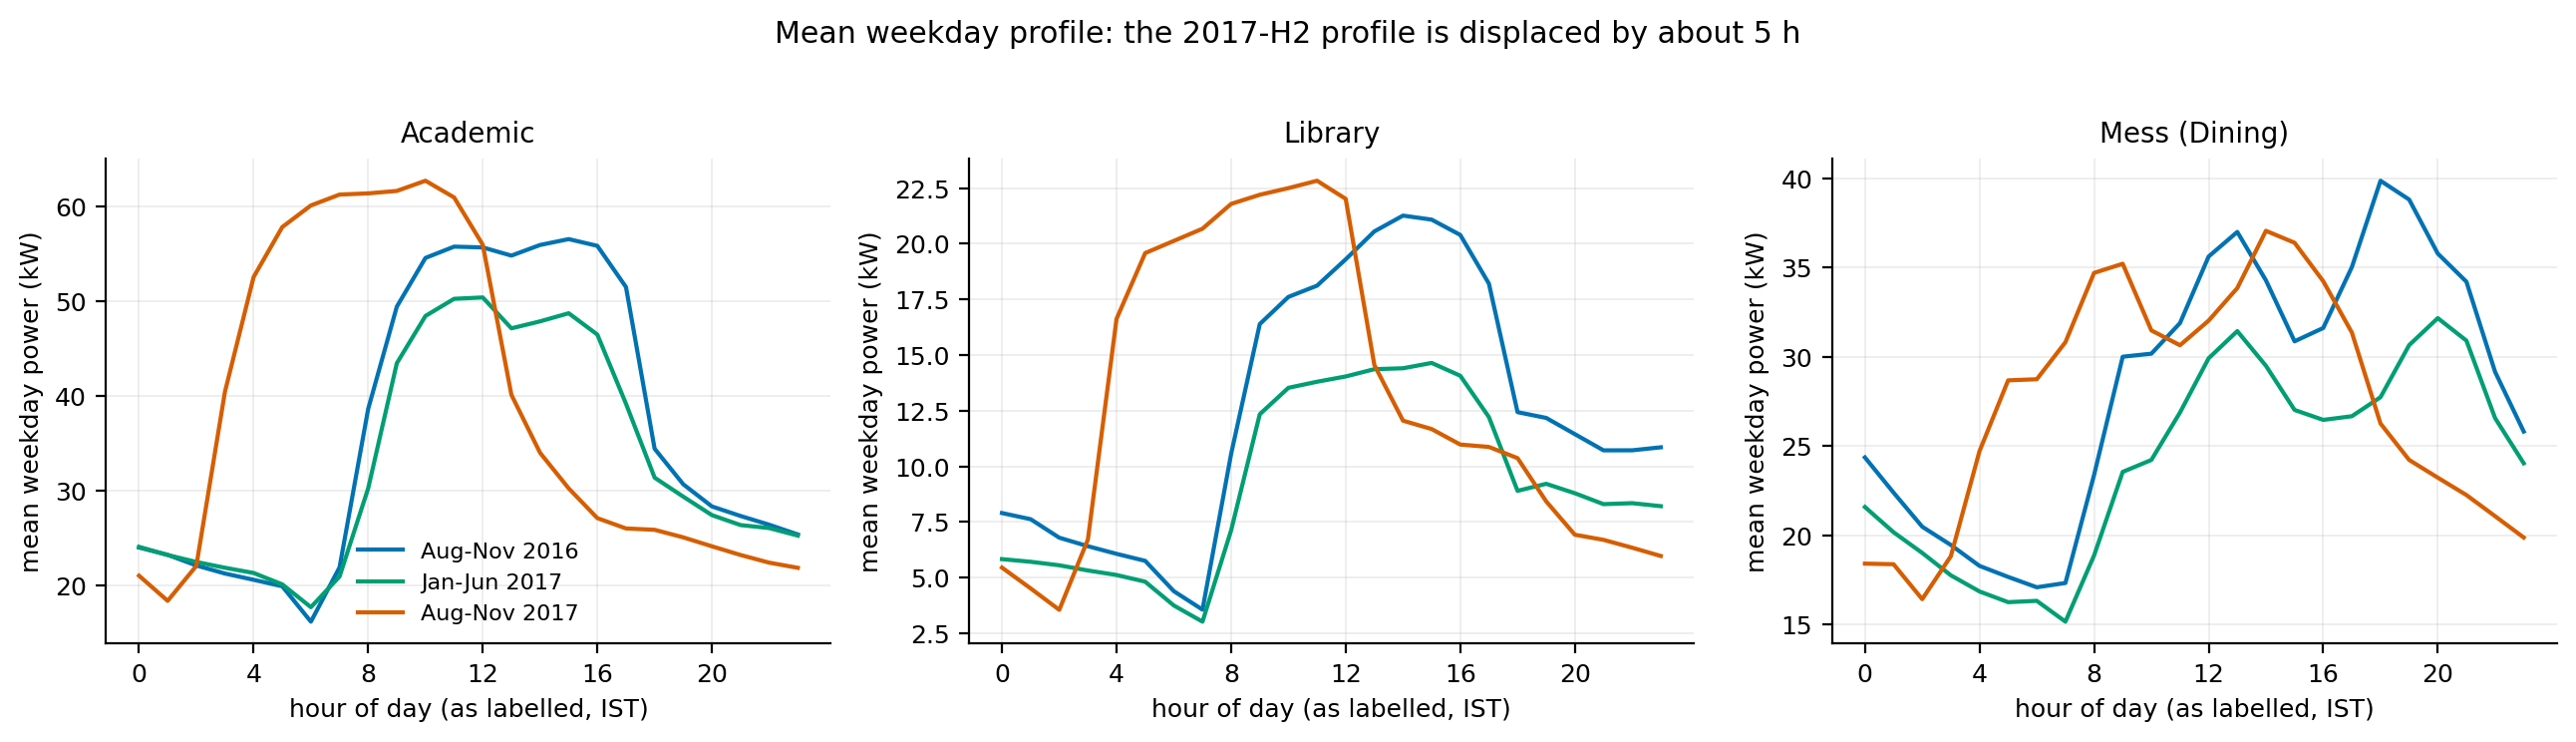
\includegraphics[width=\columnwidth]{fig19_timestamp_shift_profiles.png}
\caption{Mean weekday profiles before and after the discontinuity (hours as labelled, IST).}\label{fig:shift}
\end{figure}

\subsection{Anomaly detection}
Table~\ref{tab:an} gives the share of flagged hours. For the selected SVR model with primary features, 3.03\% of validation hours (the calibration period, out-of-sample) and 3.69\% of primary-test hours (747 hours) are flagged,
i.e.\ the thresholds transfer reasonably to the test period; after the timestamp break the rate rises to 12.34\%, which reflects the displaced timestamps (the models expect the wrong time-of-day pattern) and not consumption faults. Flags after 2017-07-08 should therefore not be interpreted.
Fig.~\ref{fig:timeline} shows the monthly share and Fig.~\ref{fig:examples} examples. Boys Hostel and Lecture have the highest primary-test rates (Table~\ref{tab:anb}); Lecture's rate is affected by its two regimes (Section~VI-C).
On matched rows, the flags of SVR with and without occupancy overlap strongly (Jaccard 0.80 on the primary test, 0.90 for Linear Regression), whereas SVR and Linear Regression agree much less (Jaccard 0.51), so the flagged set depends on the model;
the intersection of both is the more conservative list. Because the data contain no labelled faults, precision and recall cannot be computed, and the flagged hours are best described as potential anomalous consumption periods.

\begin{table}[t]
\caption{Flagged hours (\%) by model and feature set. P: energy + lagged occupancy; E: energy-only (same rows). Last column: flagged hours in the primary test.}\label{tab:an}
\centering\small
\begin{tabular}{llrrrr}
\toprule
Model & Features & Valid. & Primary test & After break & Count\\
\midrule
SVR & energy+occ. & 3.03 & 3.69 & 12.34 & 747 \\
SVR & energy-only & 3.43 & 4.19 & 11.64 & 848 \\
Linear Reg. & energy+occ. & 2.35 & 3.20 & 7.46 & 647 \\
Linear Reg. & energy-only & 2.33 & 3.25 & 7.28 & 657 \\

\bottomrule
\end{tabular}
\end{table}

\begin{table}[t]
\caption{Flagged hours (\%) per building, SVR with primary features.}\label{tab:anb}
\centering\small
\begin{tabular}{lrrr}
\toprule
Building & Valid. & Primary test & After break\\
\midrule
Academic & 4.4 & 3.5 & 24.5 \\
Boys Hostel & 3.8 & 7.3 & 13.3 \\
Facilities & 1.1 & 2.3 & 10.0 \\
Girls Hostel & 1.3 & 2.1 & 3.8 \\
Lecture & 5.3 & 9.7 & 12.2 \\
Library & 4.7 & 3.1 & 17.4 \\
Mess & 0.7 & 0.2 & 6.2 \\

\bottomrule
\end{tabular}
\end{table}

\begin{figure*}[t]
\centering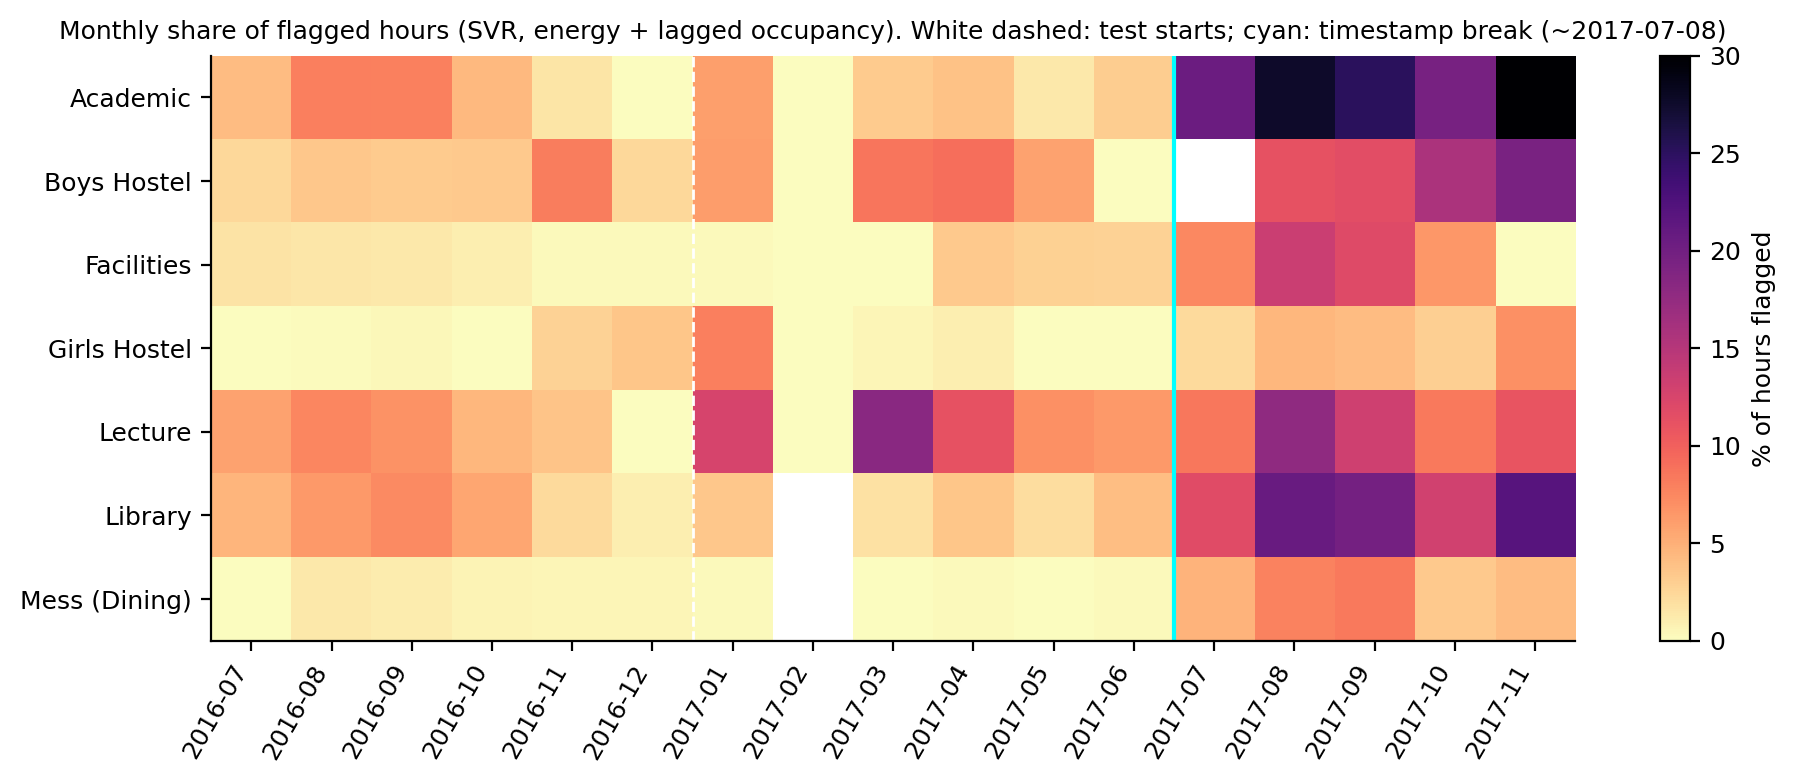
\includegraphics[width=0.9\textwidth]{fig21_anomaly_timeline.png}
\caption{Monthly share of flagged hours (SVR, primary features). The cyan line marks the timestamp discontinuity.}\label{fig:timeline}
\end{figure*}

\begin{figure}[t]
\centering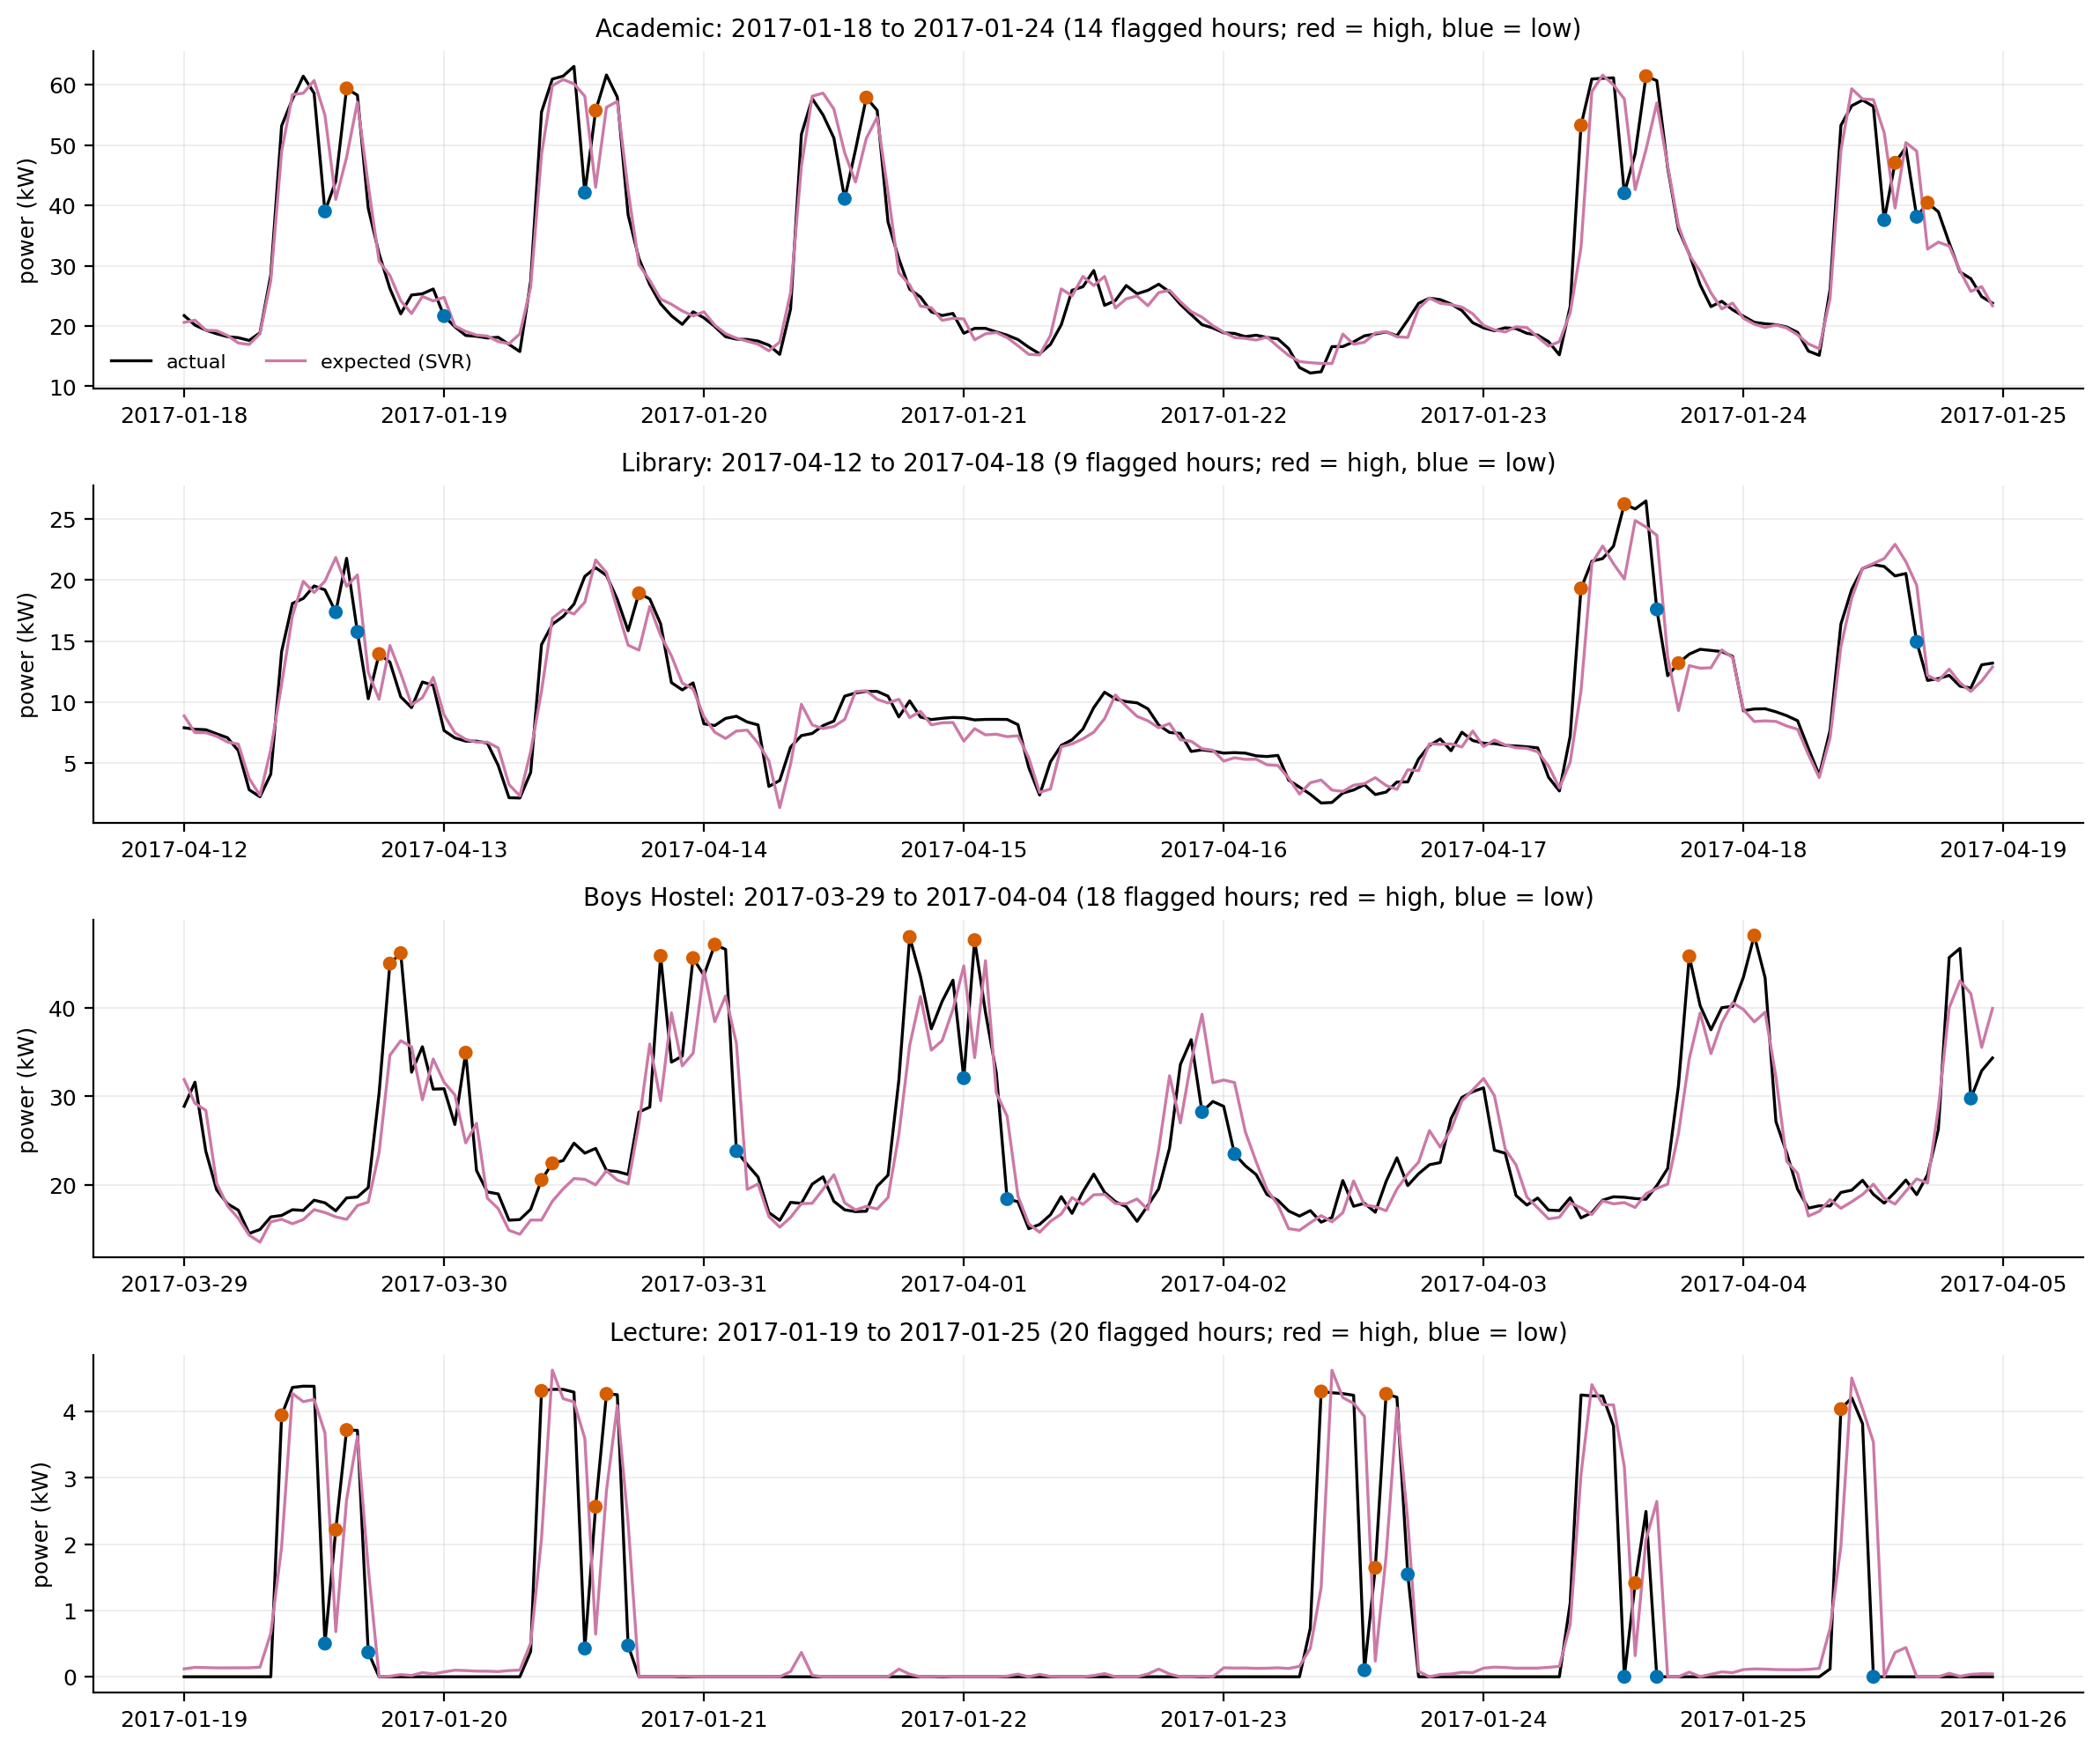
\includegraphics[width=\columnwidth]{fig22_anomaly_examples.png}
\caption{Flagged hours (markers) in the one-week primary-test windows with the most flagged hours; red: above expectation, blue: below.}\label{fig:examples}
\end{figure}

\subsection{PCA and K-Means}
The first three principal components explain 37.5\%, 16.9\% and 14.5\% of the variance, and 7 components are needed for 90\% (Fig.~\ref{fig:pca}). PC1 loads on lagged power and lagged occupancy together (a general load/occupancy level), PC2 mainly on the weekend/working-day and activity flags (calendar regime).
PCA was not used as a modelling step and no claim is made that it improves prediction.
K-Means on building-days selected $K=3$ (silhouette 0.71), but two of the three clusters consist almost exclusively of Lecture days (off days with near-zero load and on days with a high load relative to its low mean), so the clustering mainly isolates Lecture's two regimes.
Without Lecture, the silhouette favours $K=2$ (0.35, moderate structure): a cluster of higher-than-average, mostly weekday, daytime-dominated profiles and a cluster of flatter, lower-load days with more weekends (Table~\ref{tab:km}, Fig.~\ref{fig:km}). The clusters are descriptive statistical groups; no efficiency labels are assigned.

\begin{table}[t]
\caption{K-Means clusters of building-days without Lecture: days, mean load relative to the building mean, load factor, weekend share, high-activity share.}\label{tab:km}
\centering\small
\begin{tabular}{lrrrrr}
\toprule
Cl. & Days & Rel. mean & Load f. & Weekend & Act. H\\
\midrule
0 & 3{,}339 & 0.90 & 0.69 & 0.37 & 0.39 \\
1 & 1{,}311 & 1.26 & 0.61 & 0.09 & 0.52 \\
\bottomrule
\end{tabular}
\end{table}

\begin{figure*}[t]
\centering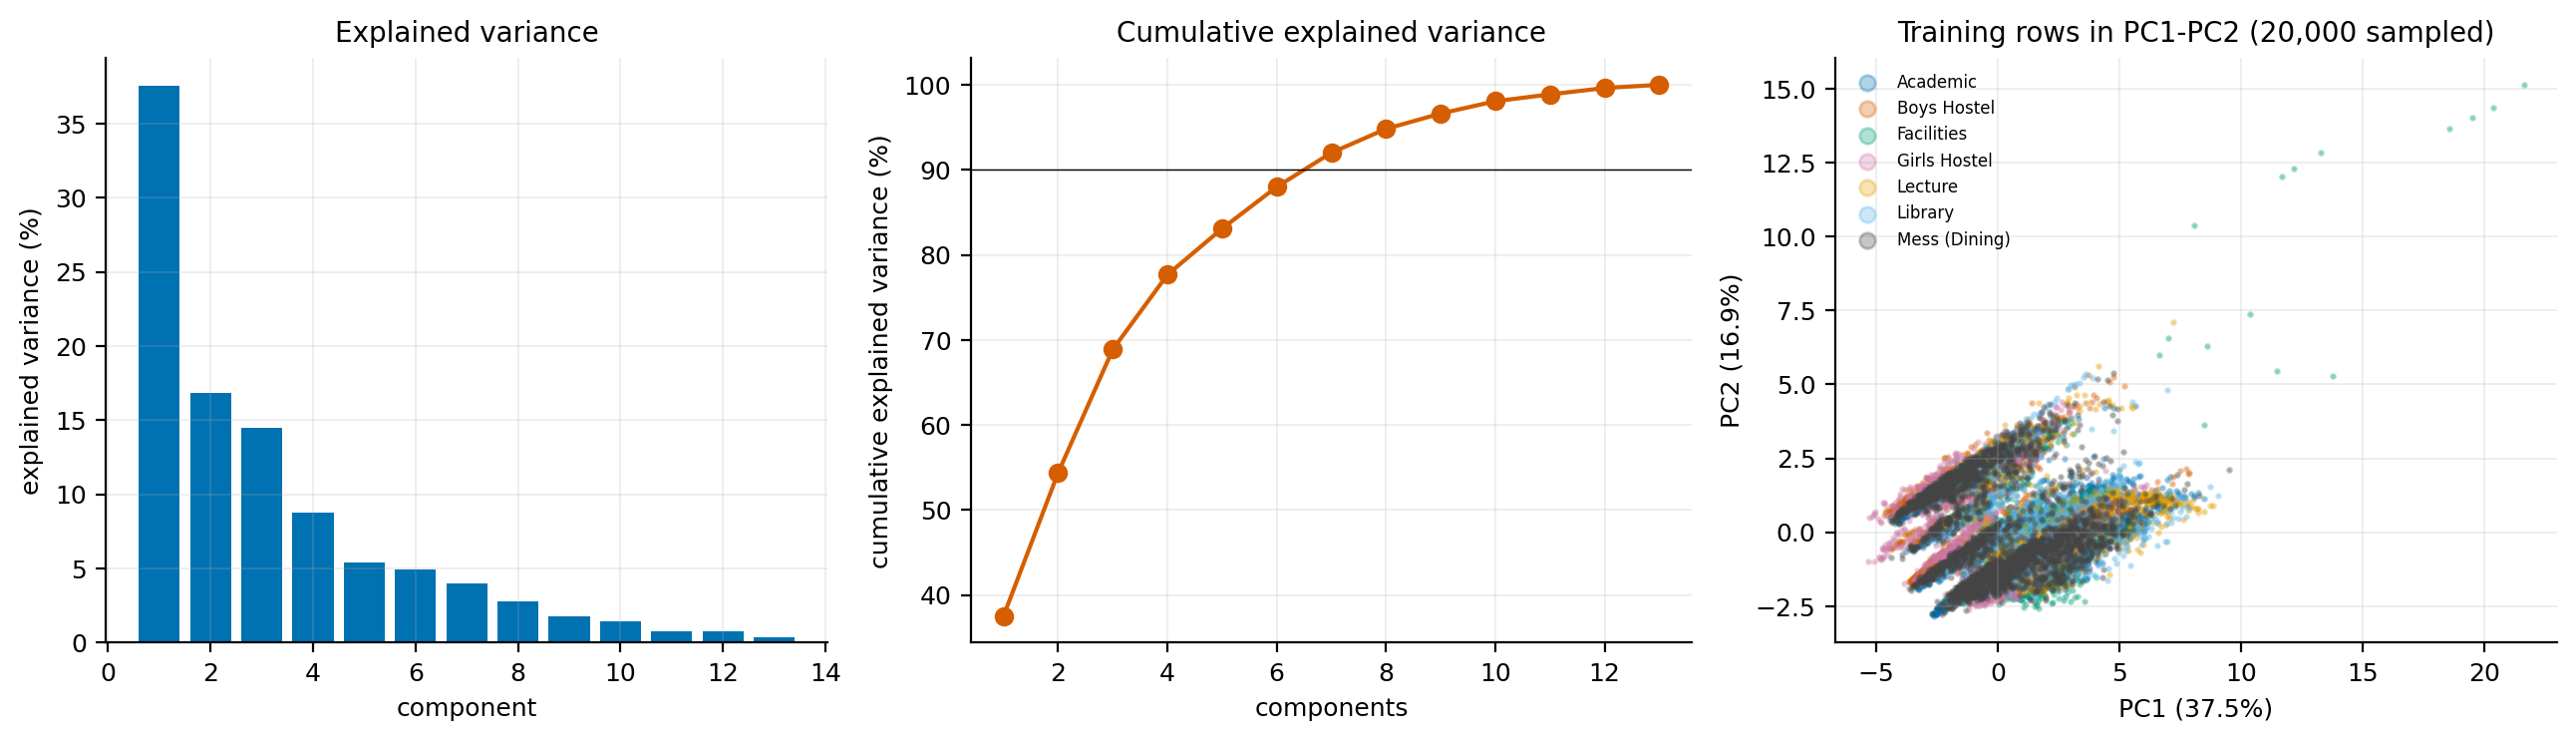
\includegraphics[width=0.95\textwidth]{fig25_pca.png}
\caption{PCA of training rows: explained variance, cumulative variance and the first two components.}\label{fig:pca}
\end{figure*}

\begin{figure*}[t]
\centering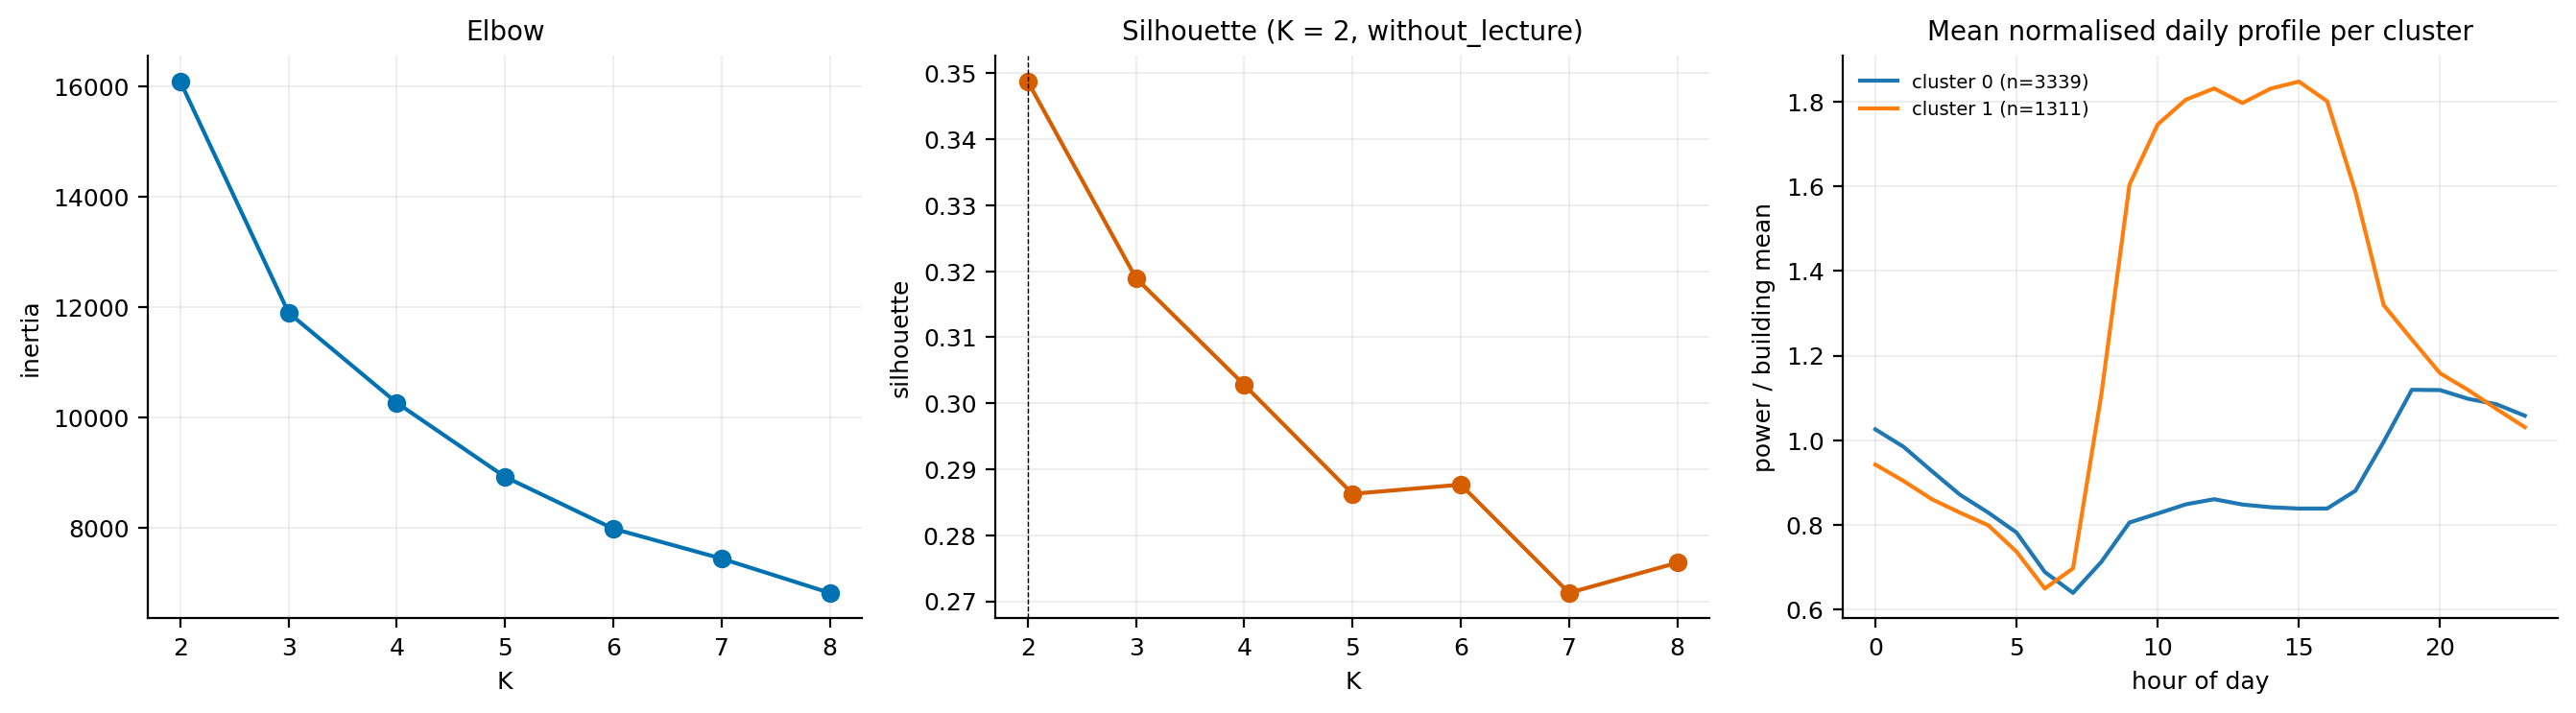
\includegraphics[width=0.95\textwidth]{fig26_kmeans_without_lecture.png}
\caption{K-Means selection (elbow, silhouette) and mean normalized daily profile per cluster, six buildings without Lecture.}\label{fig:km}
\end{figure*}

\section{Dashboard / System Implementation}
A minimal Streamlit application (\texttt{app/streamlit\_app.py}) reads only saved outputs. A sidebar selects building, model (SVR or Linear Regression), feature set and date range; a check box adds the post-break rows and a banner states the timestamp issue and that flags are not fault diagnoses.
Tabs show an overview with metrics for the selection, actual versus expected power with flagged hours, evaluation metrics (selection and frozen-model tables by period), the anomaly timeline with event table and thresholds, and CSV export of the selected hours and events.
A button re-runs the saved model file on the selected hours and reports the difference to the stored predictions. The application was tested headlessly with Streamlit's test harness for building, model, feature-set and period selections, and the server answered HTTP requests; it is a batch viewer of saved results, not a real-time monitor.

\section{Limitations}
(i) The energy timestamps after about 2017-07-08 are displaced and unresolved, which reduces the usable test period to January--July 2017 (and leaves February almost empty because of a 49-day occupancy outage).
(ii) There is no ground truth for anomalies; thresholds are statistical and flagged hours are not confirmed faults, and precision/recall cannot be assessed. (iii) Occupancy is a Wi-Fi-based proxy, absent steps cannot be distinguished from zero occupancy, and requiring occupancy lags removes about 30\% of the energy-only rows.
(iv) Weather could not be used. (v) Lecture is zero-inflated and its metrics and flags are less reliable. (vi) The hostel and library series contain long outages; a single campus is studied, so generalization to other institutions is untested.
(vii) Frozen models are trained on the training period only, SVR's selected hyper-parameters lie at the border of the searched grid, and differences between SVR and Linear Regression are small. (viii) PCA and K-Means are exploratory, and the K-Means result is dominated by Lecture.

\section{Conclusion and Future Work}
A leakage-controlled hourly pipeline for seven campus feeders was implemented and evaluated. SVR was selected on validation and had the lowest macro error on the primary test period, but its margin over Linear Regression is small, and all models improve on persistence only moderately.
Lagged occupancy did not add predictive skill. A residual-based detector calibrated on validation residuals transfers to the primary test period with a similar flag rate, and its output must be treated as a list of potential anomalous periods.
Future work: resolving the 2017 timestamp discontinuity with the dataset authors or the original logger records, reassessing the results on the corrected data, adding weather for periods where it exists, regime-aware models for Lecture, more advanced time-series models, and validation of flagged periods against maintenance records.

\bibliographystyle{IEEEtran}
\bibliography{refs}
\end{document}
